\clearpage
\section{Data Collection and Processing}
\label{sec:data-processing}

This chapter aims to describe all data preprocessing steps. After these steps, the data is ready for analysis, and machine learning models can be developed. First, we describe data collection, followed by an architectural overview of all data pipelines i.e., how the data is processed, and with what tools. Finally, we describe how each collected data source (i.e., GPS, accelerometer, and visual data) are preprocessed. 


\subsection{Data Collection}
\label{sec:data-collection}

Initially data was collected using a sensor box connected with a webcam. Specifically, an AutoPi \cite{AutoPi} was connected to the OBD-2 port of the vehicle. The OBD-2 connector is mandatory in all cars since 2004 in the EU \cite{EU1998}. Through the port, data about the vehicle internals is accessible e.g., a mechanic reading the engine status. Because the AutoPi is connected with that port, it logs various sensors such as RPM, speed, engine temperature etc. It depends on the specific vehicle what kind of data is available. Additionally, the AutoPi is equipped with sensors such as an accelerometer and GPS.

Unfortunately, there are two problems with this collection setup. First, the used webcam was unable to accurately record visual data. A webcam is designed to be used indoors and failed to deal with the variable conditions while driving (e.g., lighting, vibrations). Initially, this problem was solved by recording visual data with an external smartphone. However, there was another issue related to the accelerometer data provided by AutoPi. The sensor could only be sampled at maximum frequency of 12.5 Hz. Some initial experiments demonstrated that this low rate was not sufficient for proper data collection.

The visual data was already collected with a smartphone. Therefore, we decided to also collect accelerometer and GPS data with that same device: an Apple iPhone 12 Mini. The phone was located in a generic phone holder attached to the windshield, see figure \ref{fig:smartphone-collector}. All data collection was performed with the same vehicle, a Volkswagen Polo 2012 1.2 TSI. Data collection was done with an open-source app, which was slightly modified and deployed on the smartphone.\footnote{See \cite{ios_logger} for modified fork and \cite{ios_logger_original} for original. Main modification is to keep the smartphone from sleeping while collecting data.} With this app, the following data is collected:
\begin{itemize}
\item Visual data: recorded in 1280 x 720 at 30 frames per second.
\item Accelerometer data: sampled at 100 Hz.
\item Location data: sampled at 1 Hz and consisting of GPS coordinates, travel heading, and traveling speed.
\end{itemize}


\begin{figure}[H]
\begin{center}
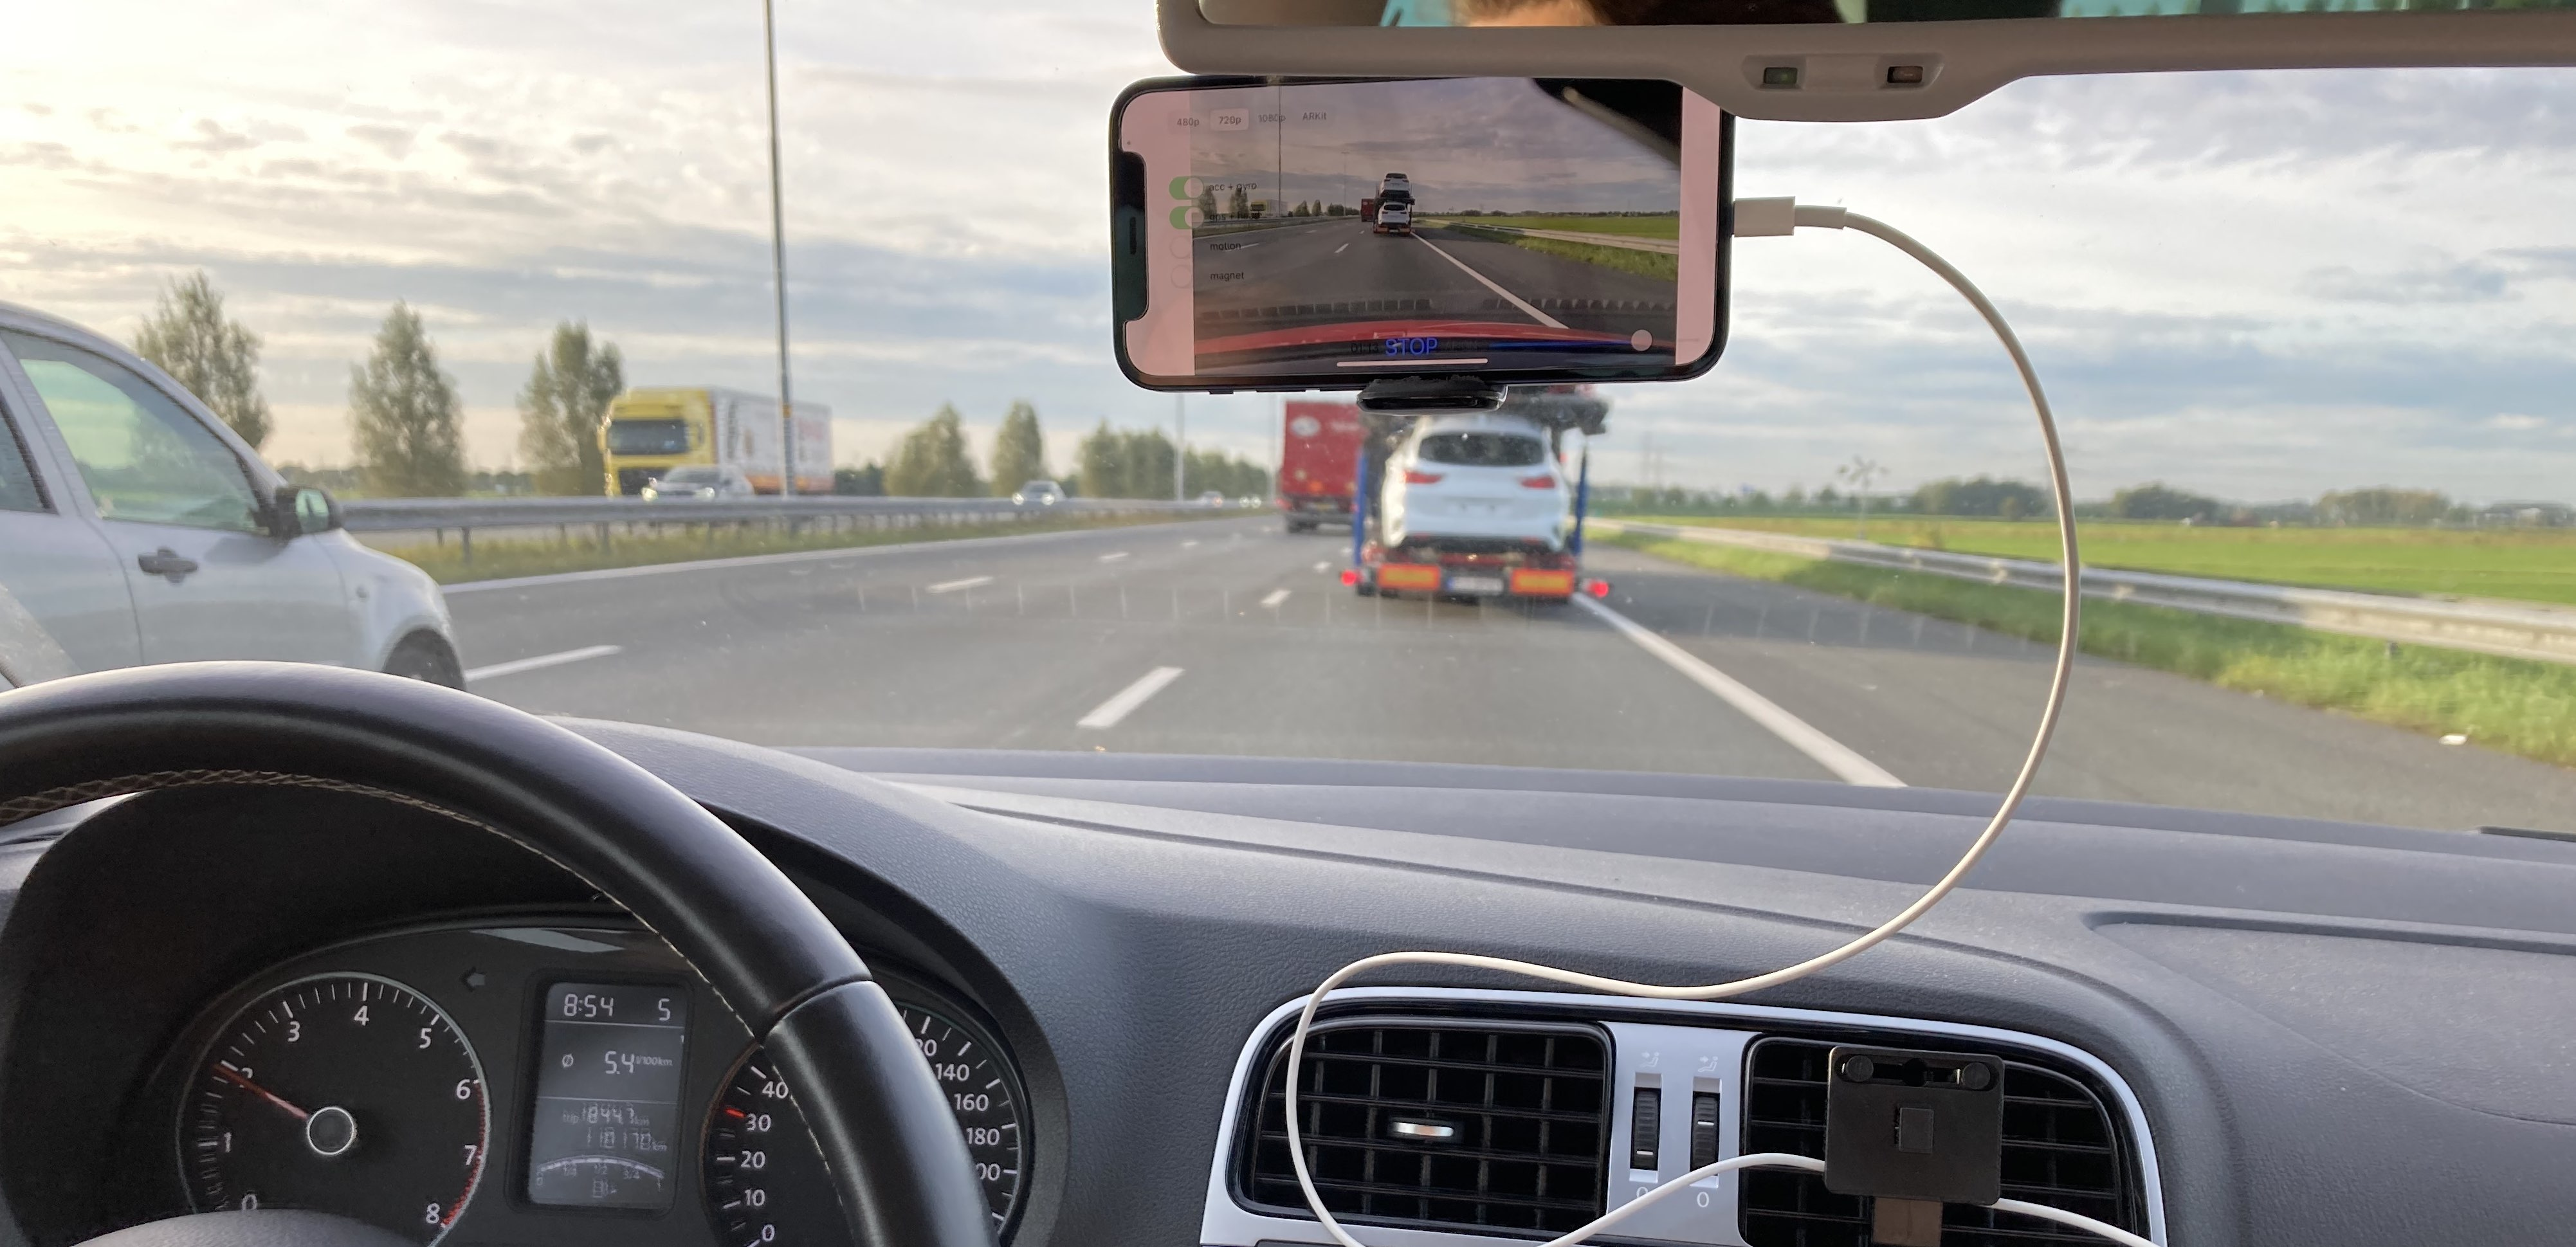
\includegraphics[width=0.95\textwidth,keepaspectratio]{images/4_data/smartphone-setup.jpg}
\end{center}
\captionsetup{width=.90\textwidth}
\caption{Setup of collecting data. An Apple iPhone 12 Mini is located in a generic smartphone holder, attached to windshield of a Volkswagen Polo 2012 1.2 TSI.}
\label{fig:smartphone-collector}
\end{figure}


\subsection{Data Platform Architecture}
The collected data is systematically processed through various data pipelines. All data pipelines combined are holistically presented as a \textit{data platform architecture}. The developed data pipelines are designed to be executed using cloud services. Reason for this choice is twofold. First, some data operations take a long time to be processed. Using cloud services processing of the data is more efficient, i.e., due the availability of highly scalable resources. For instance, multiple data pipelines can run in parallel. Secondly, the developed solution is to be deployed within the existing application PRM (see section \ref{sec:assetworx}). With this architecture the solution is easily integrated within the PRM software.

Implementation and execution of the data platform uses Google Cloud Platform (GCP). It uses the following services provided by GCP: Cloud Storage, BigQuery - a data warehousing solution, and Kubernetes - a platform for executing container workloads. Orchestration of all data pipelines is done using Prefect \cite{Prefect}, a ``data workflow automation tool''. This tool is designed to orchestrate large scale workflows for data processing. However, it also provides an easy to use library to create and run data pipelines locally.

The solution uses a modern data platform architecture with loosely coupled layers. A data architecture is either modelled based on the used data sources, or on the specific ``areas'' (or maturity) of the data. In this case, the latter approach is used. Maturity refers to the readiness of consumption of that respective data. Data comes in its raw form into the data platform (landing area), but often needs some transformations (i.e., cleaning, deduplication) to make it ready for consumption (production area).  Figure \ref{fig:data-platform-architecture} shows an overview of the data platform, which is composed of three major layers: ingestion, storage, and processing.

\begin{figure}[H]
\begin{center}
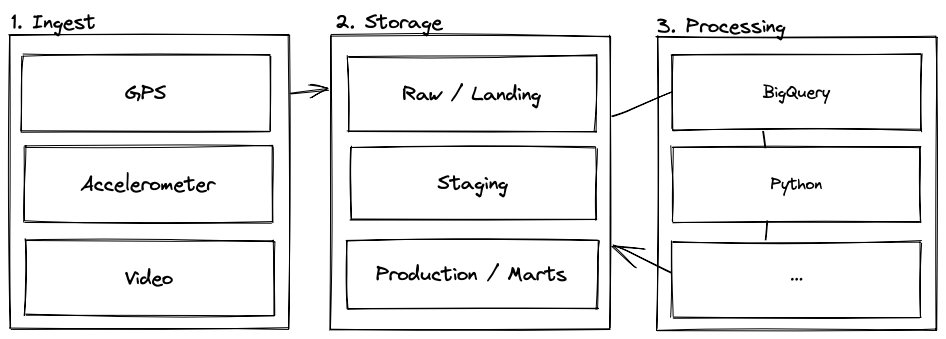
\includegraphics[width=0.85\textwidth,keepaspectratio]{images/4_data/data-platform.png}
\end{center}
\captionsetup{width=.90\textwidth}
\caption{Overview of data platform architecture.}
\label{fig:data-platform-architecture}
\end{figure}

\begin{enumerate}
\item Ingestion Layer: it sends the data to the data platform. Data is manually pulled from the smartphone to a laptop. From this laptop the data is uploaded to the cloud platform using automated scripts. Note, to ensure privacy concerns, visual data is first anonymized to remove any personal identifiable data (e.g., cars containing license plates, persons).
\item Storage Layer: data is stored in the data platform in two services: BigQuery - a managed data warehouse solution and Cloud Storage - a generic object store. Within these two services, the data is split in three layers denoting the maturity of the data.
\begin{enumerate}
\item Raw / landing: it contains data in the form collected by the smartphone.
\item Staging: an intermediate layer to preprocess data.
\item Production / marts: it contains data ready to be analyzed data and train the models.
\end{enumerate}
\item Processing Layer: it consumes data from the storage layer and processes it. Some processing steps are implemented in SQL and executed in BigQuery; whereas others are implemented in Python (using Prefect) and executed locally or in the Kubernetes cluster.
\end{enumerate}


A complete overview of all data pipelines is given in appendix \ref{sec:appendix-a-data-pipelines}. The appendix describes the input and output of each data pipeline, and where it is executed (e.g., BigQuery, or Kubernetes). Additionally, a cohesive flowchart is shown. The rest of this chapter describes the data pipelines from a functional perspective.

\subsection{GPS Data}
GPS data describes the location of the vehicle in coordinates. Specifically, the coordinates are recorded as latitude and longitude (i.e., WGS84 standard \cite{wgs84}). The data is sampled at 1 Hz. GPS data is further processed to compute distinctive trips, speed and heading information of the travelling vehicle.

\begin{figure}[ht]
\begin{center}
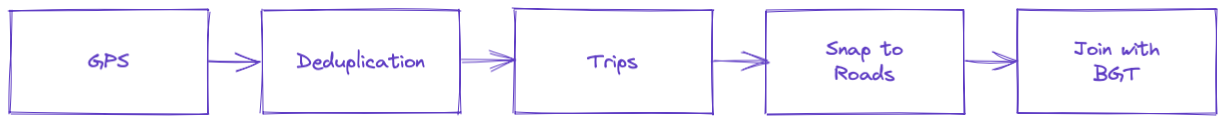
\includegraphics[width=0.95\textwidth,keepaspectratio]{images/4_data/processing-overview-gps.png}
\end{center}
\captionsetup{width=.90\textwidth}
\caption{Figure displaying all processing operations for GPS data.}
\label{fig:processing-overview}
\end{figure}



\subsubsection{Determine Trips}
The GPS sensor records the location of the vehicle. After ingestion, this data is stored in a raw form on Google Cloud Storage (GCS), as json lines. This is a file format where each line in the file is a single json document. Within this document the location of the vehicle is recorded with the respective time. From Cloud Storage the data is ingested into BigQuery, which detects duplicated trips with the algorithm described below. Each trip has an unique identifier that is used to combine different data sources e.g., finding the accelerometer data for a specific trip.

\begin{enumerate}
\item Deduplication: the GPS sensor always records location data. If the car is standing still (e.g. traffic light), the data is still recorded, resulting in duplicate records. The first step is to deduplicate the data. This is done by selecting the first record for each unique location in subsequent time series. See listing \ref{list:deduplication} for psuedo implementation.
\item Delta calculation: the algorithm computes the time and distance difference for each record.
\item Split trips: trips are detected by splitting the records where the ``dwell time'' is higher then some threshold. Dwell time is the time period when the vehicle on the same location. From literature, we find that 120 seconds is often used as threshold \cite{Wolf2001}. See listing \ref{list:split-trips} for psuedo implementation.
\item Reset trips: for each first record of a trip, the delta time and distance is reset to zero.
\item Cleanup trips: the algorithm keeps only trips with more than five records and at least 500 meters travelled to cleanup invalid data.
\end{enumerate}

\begin{lstlisting}[language=Python, caption={Psuedo implementation of deduplicating GPS coordinates.}, label={list:deduplication}]
def deduplicate(source_data: list):
    deduplicated = []
    for x in source_data:
        # For all following records, find first record that
        # has different coordinate.
        x_at = index_of(x)
        for y in source_data[x_at:]:
            if x.coord != y.coord:
                deduplicated.append(x)
                break
                
    return deduplicated
\end{lstlisting}
    
\begin{lstlisting}[language=Python, caption={Psuedo implementation of splitting GPS data into trips.}, label={list:split-trips}]
def split_trips(source_data: list):
    # Period in seconds after which new trips are detected
    dwell_time = 120
    trip_id = 0

    # Iterate through all data points
    previous = source_data[0]
    for x in source_data[1:]:
        # New trip is detected after period of dwell
        if previous.timestamp - x.timestamp > dwell_time:
            trip_id += 1
        
        # Appoint trip_id to GPS record
        x.trip_id = trip_id
        previous = x
\end{lstlisting}


\begin{figure}[H]
  \centering
  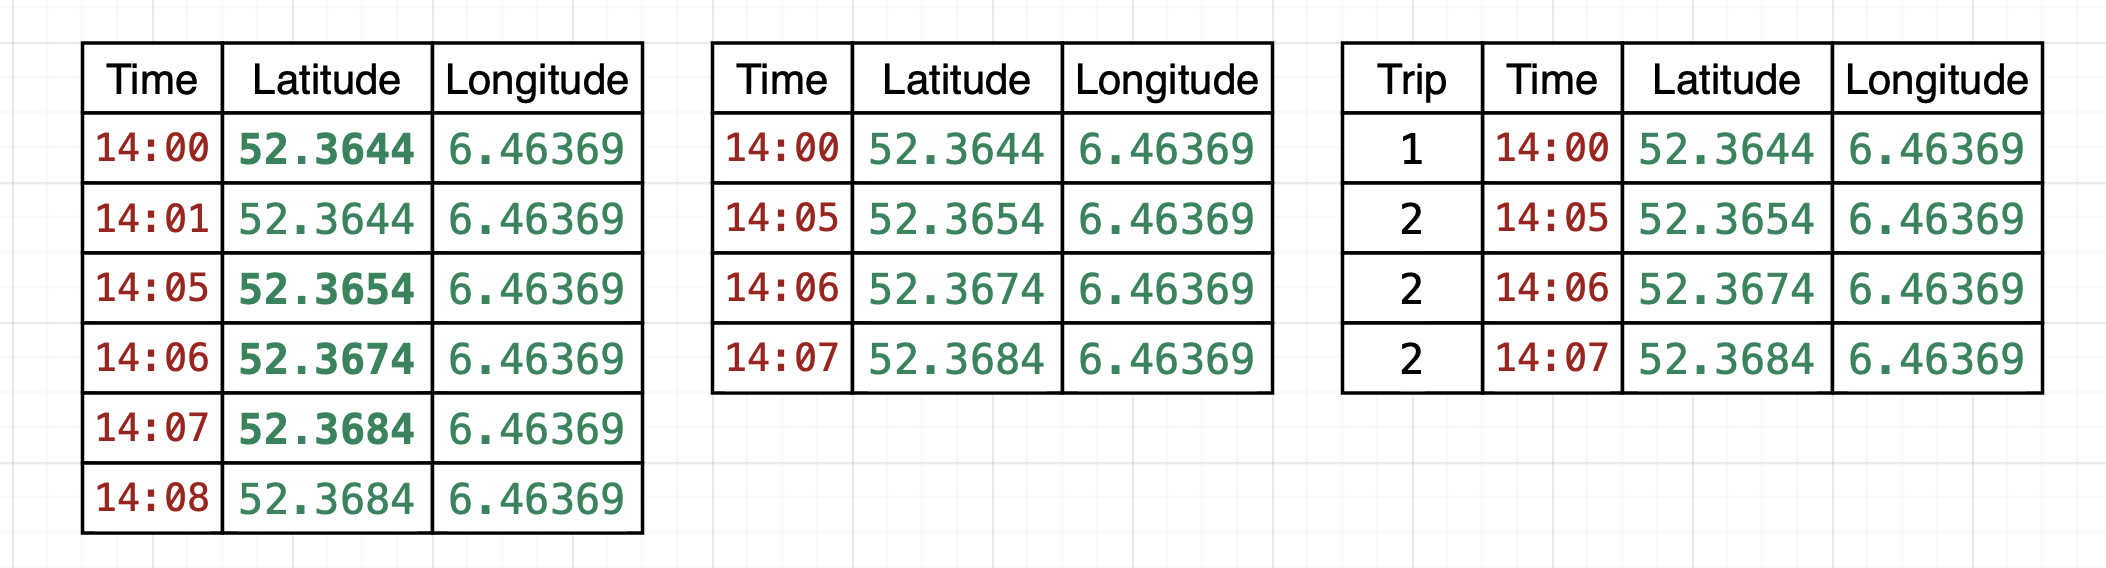
\includegraphics[width=0.95\linewidth]{images/4_data/trip-detection.png}
  \captionsetup{width=.90\textwidth}
  \caption{Example of trip deduction algorithm. Left shows original data, center shows after deduplicating based on the location, right shows the resulting trips.}
  \label{fig:test2}
\end{figure}




\subsubsection{Snap Trips to Roads}
GPS data is generally regarded as noisy. The accuracy of the sensor varies over time; thus, some coordinates are aligned with roads, while other samples are outside them (see figure \ref{fig:snap-trips}). This is an issue when processing data further. In our case, we want to join GPS data with road information (further described below) by snapping GPS coordinates to actual roads. To this aim, we use an external service named ``Snap Points to Roads'' from Bing Maps \cite{Snap-Points-to-Roads}. However, we could leverage alternatives as well. For instance Google Maps offers a similar API, but costs more.

Usage of these services is straightforward. For each trip, all coordinates are send to the API. The service responds with a a list of modified coordinates snapped to the roads. The service automatically derives the driving direction based on the timestamps. The driving direction is used to correctly snap the coordinate to the right lane. Thus, if a coordinate is erroneously recorded on the oncoming lane, the service corrects for it.

\begin{figure}[H]
\begin{center}
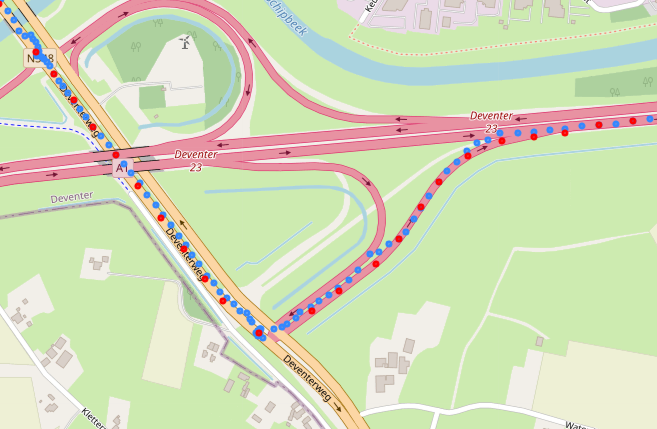
\includegraphics[width=.85\textwidth,keepaspectratio]{images/4_data/snap-trips.png}
\end{center}
\captionsetup{width=.90\textwidth}
\caption{Display of snapping coordinates to roads. The blue dots are the measured GPS coordinates, and the red dots are the inferred coordinates by external service. Note that some of the blue dots are on the wrong lane or beside any roads.}
\label{fig:snap-trips}
\end{figure}


\subsubsection{Link Trip Coordinates with Road Sections}
\textit{Basisregistratie Grootschalige Topografie} (BGT) is the registry of ``large-scale objects in the public space'' in the Netherlands. This registry records all geographic locations of so called large-scale objects. These include roads, buildings, and estate. The BGT is regulated by law and is mandatory for governments to use and maintain while operating in the public space \cite{BGT}. The BGT registers roads as ``road sections''. The size of a section varies to a single street bump in a town, to several hundred meters of highway. Road sections are annotated with various types of attributes. In this case, we are interested in the type of road: concrete, asphalt, or brick. Brick roads are common in urban areas in the Netherlands and generate significant vibrations, which might need to be filtered out. 

The road snapped coordinates are used to find the respective road section from the BGT. For each GPS record it finds the road section where that coordinate is in contained. See also listing \ref{list:join-bgt} for psuedo implementation.


\begin{lstlisting}[language=Python, caption={Psuedo implementation of joining GPS data with road sections.}, label={list:join-bgt}]
def join_gps_with_bgt(gps_data: list, bgt: list):
    for gps in in gps_data:
        for road_section in bgt:
            if road_section.contains(gps.coordinate):
                gps.road_section = road_section
\end{lstlisting}


\subsection{Accelerometer Data}
Accelerometer measures acceleration, the change of velocity over time. In the smartphone the sensor measures acceleration in three axis: longitudinal (X), lateral (Y), and vertical (Z) axes. The output is in G-forces, where $1 G = 9.81m/s^2$. In stationary position, the accelerometer always measures 1G on the vertical axis due gravitational pull of the earth. Acceleration data describes the vibrations of the vehicle. However, before the data can be used, it needs to be pre-processed. The most important prepocessing step is the alignment of sensor orientation with the direction of the vehicle. All processing steps are described below.

\begin{figure}[H]
\begin{center}
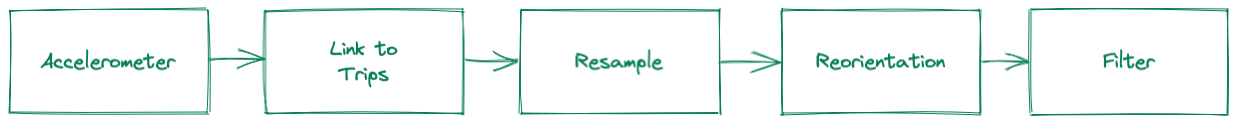
\includegraphics[width=0.95\textwidth,keepaspectratio]{images/4_data/processing-overview-accelerometer.png}
\end{center}
\captionsetup{width=.90\textwidth}
\caption{Figure displaying all processing operations for accelerometer data.}
\label{fig:processing-overview}
\end{figure}


\subsubsection{Resampling}
Resampling the data ensures a constant sampling frequency. This is necessary for further signal processing operations such as calculating FFT or filtering noise. The effect of resampling is shown in figure \ref{fig:accelerometer-resampling}, which represents the data collected with AutoPI, as the effect is less noticeable with the more consistent data from the smartphone. The top blue graph shows the raw readings from the accelerometer. The bottom red graph shows the resulting data after re-sampling. Note that the interval between readings of the top graph vary, whereas the bottom is uniformly spaced.

Resampling of the data is done by fitting a B-spline curve for all the known samples. From this spline, the data points are uniformly sampled at the expected frequency of 100 Hz. To perform these calculations, the open-source Python library scipy is used \cite{scipy}. See listing \ref{list:resampling} for psuedo implementation.


\begin{figure}[H]
\begin{center}
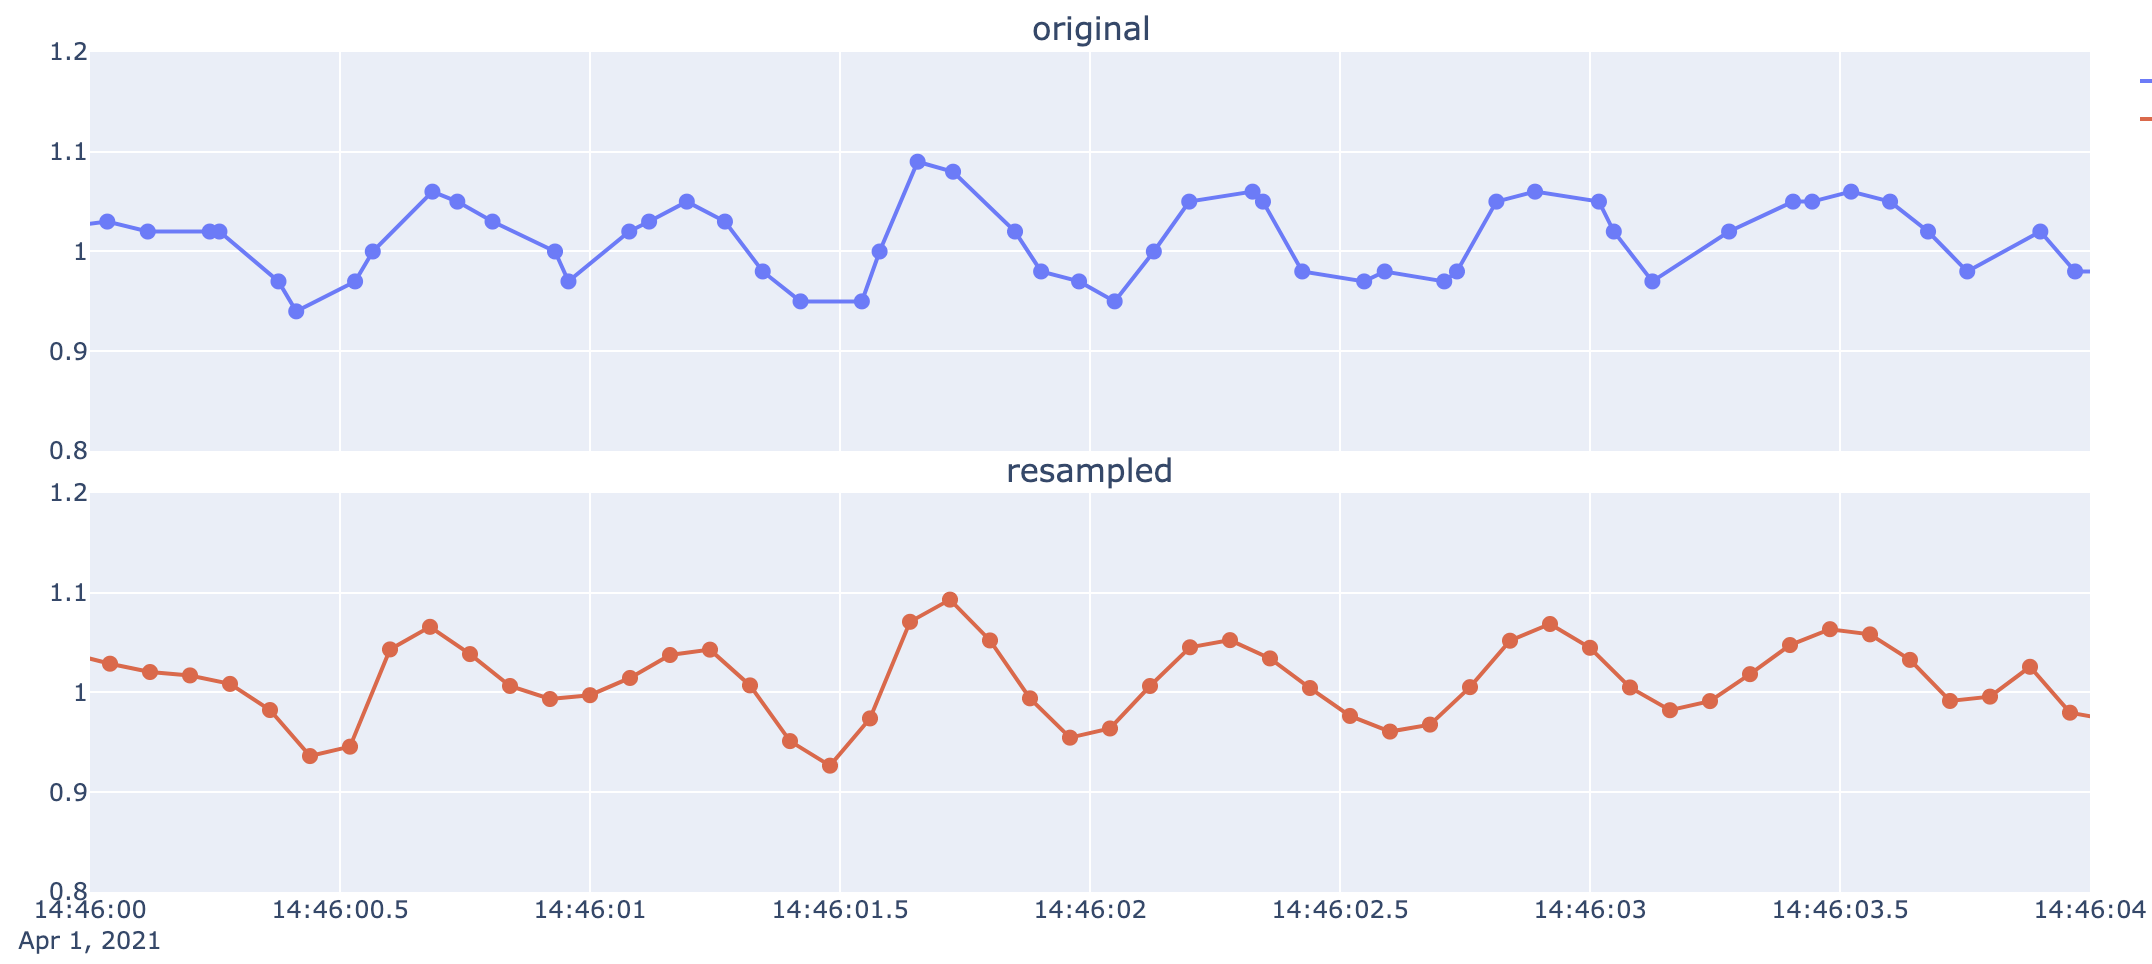
\includegraphics[width=.95\textwidth,keepaspectratio]{images/4_data/accelerometer-resampling.png}
\end{center}
\captionsetup{width=.90\textwidth}
\caption{Top graph displays the raw data from the accelerometer. Bottom graph displays the accelerometer data after re-sampling. Note this example is made on data from AutoPi, where the effect is more prominent.}
\label{fig:accelerometer-resampling}
\end{figure}


\begin{lstlisting}[language=Python, caption={Psuedo implementation of resampling accelerometer data.}, label={list:resampling}]
from scipy import interpolate

def resample_accelerometer(acc_data):
    # Create uniform timestamp ticks
    x_min = round(acc_data.timestamp.min().seconds)
    x_max = round(acc_data.timestamp.max().seconds)
    x_resampled = list(x_min, x_max, 1 / 100)

    # For all accelerometer axes
    for var in ['x', 'y', 'z']:
        # Fit a B-spline using scipy
        tck = interpolate.splrep(acc_data['timestamp'], acc_data[var])
        # Sample uniformly from the spline
        resampled = interpolate.splev(x_resampled, tck)
        
        # Overwrite the data
        acc_data[var] = resampled
\end{lstlisting}



\subsubsection{Reorientation}
\label{sec:reorientation}

The coordinate system of the accelerometer may not coincide with that of the vehicle. In other words, when the vehicle drives over a bump we expect to see a acceleration in vertical axes. However, when the vehicle is not aligned, the acceleration is shown on a different axes or as a product of axes. There are two causes for this misalignment. First, the orientation of the sensor in the smartphone is not known, making it hard to align it correctly. Secondly, we cannot expect to place the smartphone always equally in the holder. Before any data can be analyzed, the coordinate system of the accelerometer must be aligned with that of the vehicle. Therefore, we develop a method to automatically align the coordinate systems and making it possible to generalize data collection to any vehicle and accelerometer sensor. This process is inspired by \authorref{accelerometer_alignment} and actually is also applied in \authorref{Wu2020}. See listings \ref{list:calculate_mean_stationary_readings} - \ref{list:realign_vertical} for pseudo implementation of these processing steps.

It consists of two steps. First, the coordinate system is aligned on the vertical Z-axes using a rotation matrix $R_z$. Subsequently, the horizontal plane is aligned using a rotation matrix $R_x$. Calculating these rotation matrices is done by measuring the accelerometer sensor $a_s$ when a known force is exerted on the vehicle, $a_v$. Using Euler angles we can calculate the rotation matrix to align the force $a_s$ to that of the known force $a_v$. In the figure \ref{fig:align-vectors} the two-step method is visually presented.


\begin{figure}[H]
\begin{center}
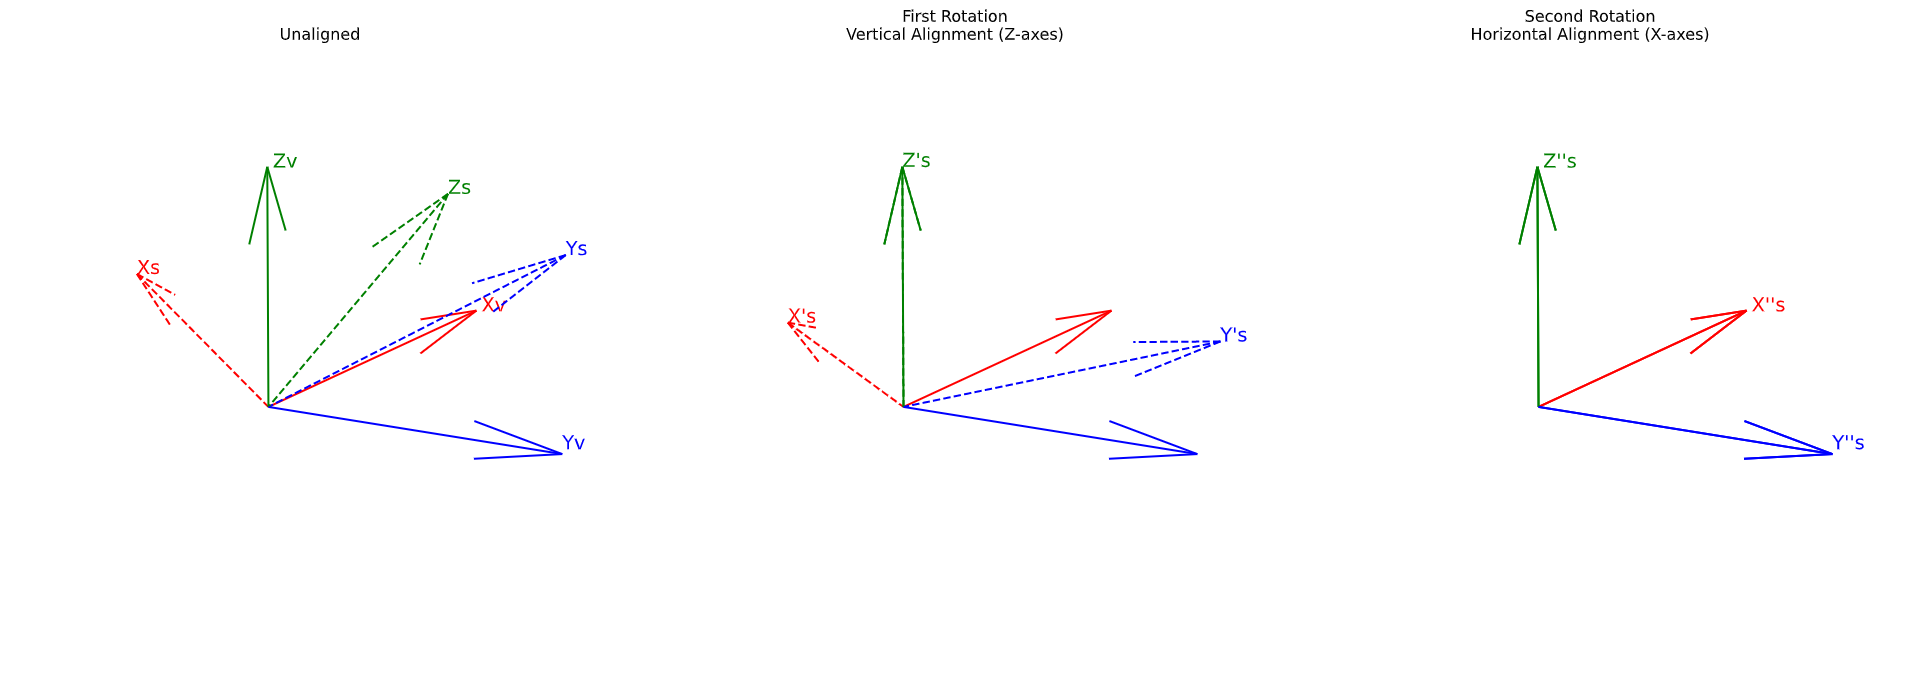
\includegraphics[width=0.95\textwidth,keepaspectratio]{images/4_data/accelerometer-alignment.png}
\end{center}
\captionsetup{width=.90\textwidth}
\caption{Figure displaying the process of aligning the axes. Zv is the Z-axes for the vehicle, Zs is the Z-axes for the sensor. Left: shows the original, unaligned situation. Middle: shows the situation after aligning the Z-axes. Right: shows situation after aligning the X-axes.}
\label{fig:align-vectors}
\end{figure}


For the first step, aligning the vertical Z-axes, the known force is the gravity of the earth. When the vehicle is stationary, the expected force is $a_v = (0, 0, 1G)$. Stationary points are found by querying the GPS data when the car is not moving. Ideally, only accelerometer data is used when the vehicle is on a level surface. As we do not have access to this information, we rely on taking the average of many samples, as it can be assumed that on average the vehicle is mostly stationary on a flat surfaces. This assumption seems plausible in the Netherlands, where the country is largely flat. The rotation matrix $R_z$ is calculated to align vector $a_s$ onto vector $a_v$.

The second step is to align the coordinate system in the longitudinal X-axes. Again, we take readings of the accelerometer when a certain force is expected. In this case when the car is braking, the expected acceleration is $a_v = (-x, 0, 1G)$, where $x$ depends on the deceleration of the vehicle. Braking windows are selected based on the derived speed from the GPS coordinates. In this step we calculate a two dimensional rotation matrix $R_x$ to align vector $a'_s$ onto vector $a_v$ in the longitudinal X-axes. $a'_s$ refers to the measured acceleration after applying the first rotation.

\begin{figure}[H]
\begin{minipage}{0.45\textwidth}

\begin{flalign*} 
\text{Let } v &= a_s \times a_v \\
\text{Let } c &= a_s \cdot a_v \\
\text{Let } skew &=
\begin{bmatrix} 0 & -v_3 & v_2 \\ v_3 & 0 & -v_1 \\ -v_2 & v_1 & 0 \end{bmatrix} \\
R_z &= I + skew + skew^2 \frac{1}{1 + c} 
\end{flalign*}

\end{minipage}
\begin{minipage}{0.45\textwidth}

\begin{flalign*} 
\sin \theta &= a'_s \times a_v \\
\cos \theta &= a'_s \cdot a_v \\
R_x &= \begin{bmatrix} \cos \theta & -\sin \theta & 0 \\ \sin \ \theta & \cos \theta & 0 \\ 0 & 0 & 1 \end{bmatrix} \\
\end{flalign*}

\end{minipage}

\captionsetup{width=.90\textwidth}
\caption{Equations to calculate the rotation matrix. Left, calculates the 3D rotation matrix to align the Z axis. Right, is the second rotation matrix to rotate in the X axis \cite{rotation_matrix}.}
\label{eq:rotation-matrix}
\end{figure}

\begin{minipage}{.95\textwidth}
\begin{lstlisting}[language=Python, caption={Pseudo implementation of calculating stationary readings.}, label={list:calculate_mean_stationary_readings}]
def calculate_mean_stationary_readings(acc_data):
    # Minimum amount of seconds the car is stationary
    stationary_window = 3

    # Query GPS data for given trip
    gps_data = query_gps(acc_data.trip_id) 
    
    # Find stationary windows
    stationary_moments = []
    previous = gps_data[0]
    for gps in gps_data[1:]:
        # Note, after deduplicating each GPS record registers
        # how long that GPS location was measured, i.e., how
        # long the vehicle is at this point.
        if gps.delta_seconds > stationary_window:
            stationary_moments.append(gps.timestamp)
        
        previous = gps
            
    # Calculate mean accelerometer reading
    readings = []
    for acc in acc_data:
        for stationary in stationary_moments:
            if  acc.timestamp >= stationary and 
                acc.timestamp <= stationary + stationary_window:
                    readings.append(acc)
    
    return mean(readings)
\end{lstlisting}
\end{minipage}

\begin{minipage}{.95\textwidth}
\begin{lstlisting}[language=Python, caption={Pseudo implementation of calculating mean readings while the vehicle is braking.}, label={list:calculate_mean_braking_readings}]
def calculate_mean_braking_readings(acc_data):
    # Minimum amount of seconds the car is stationary
    stationary_window = 3

    # Query GPS data for given trip
    gps_data = query_gps(acc_data.trip_id) 
    
    # Find consecutive records where the speed is declining
    braking_moments = []
    previous = gps_data[0]
    
    # First record in consecutive window that starts braking
    start_braking = None
    for gps in gps_data[1:]:
        if gps.speed <= previous.speed:
            # Set first record 
            if start_braking is None:
                start_braking = gps
        
        # Speed not declining anymore, but we have found at least one braking record
        elif start_braking is not None:
            # Register the start and end timestamp
            braking_moments.append(start_braking.timestamp, gps.timestamp)
            start_braking = None
            
        previous = gps
            
    # Calculate mean readings, see listing `\ref{list:calculate_mean_stationary_readings}`
    return calculate_mean(braking_moments)
\end{lstlisting}
\end{minipage}

\begin{minipage}{.95\textwidth}
\begin{lstlisting}[language=Python, caption={Pseudo implementation of reorienting accelerometer data vertically. Implementation for the second rotation matrix is similar. Except then we use mean readings while braking, and calculate a 2D rotation matrix.}, label={list:realign_vertical}]
def realign_vertical(acc_data):
    # Get stationary readings (a_s)
    stationary_readings = calculate_mean_stationary_readings(acc_data)
    # The expected force we want to orient towards, i.e., 1G vertical force
    target_vector = (0, 0, 1)

    # Calculate rotation matrix
    R = calculate_3d_rotation(stationary_readings, target_vector)
    
    # Apply it for each element
    return R.dot(acc_data)
\end{lstlisting}
\end{minipage}




\subsubsection{Noise filtering}
Accelerometer data is prone to noise. As is common with signal processing, data is first passed through a filter to obtain a clearer signal. Noise in the signal comes from vibrations generated by vehicle while driving. Existing research uses a variety of different filter configurations to clean the data. Some apply a low-pass Butterworth filter \cite{Gupta2020}, whereas other researches use a high-pass Butterworth filter \cite{Wu2020, Janani2020}. Refer back to section \ref{sec:butterworth-filter} for explanation of Butterworth filter. As the configuration differs per research, we assume it depends per application. 

In figure \ref{fig:filter}, various configurations of a 5th-order Butterworth filter are displayed. Butterworth filter is applied using the \code{butter} and \code{lfilter} functions from the computational library SciPy \cite{scipy}. The top left (blue) plot shows the original signal while driving over a manhole. The other plot shows the resulting signal after applying a specific configuration. For instance, the middle right (orange) is after passing the data through a high pass filter with cut-off at 2 Hz. Meaning that all frequencies below 2 Hz are filtered out. As this signal seems most clean, we use this configuration as an initial starting point. In future, other types of configurations could be applied to optimize performance.


\begin{figure}[H]
\begin{center}
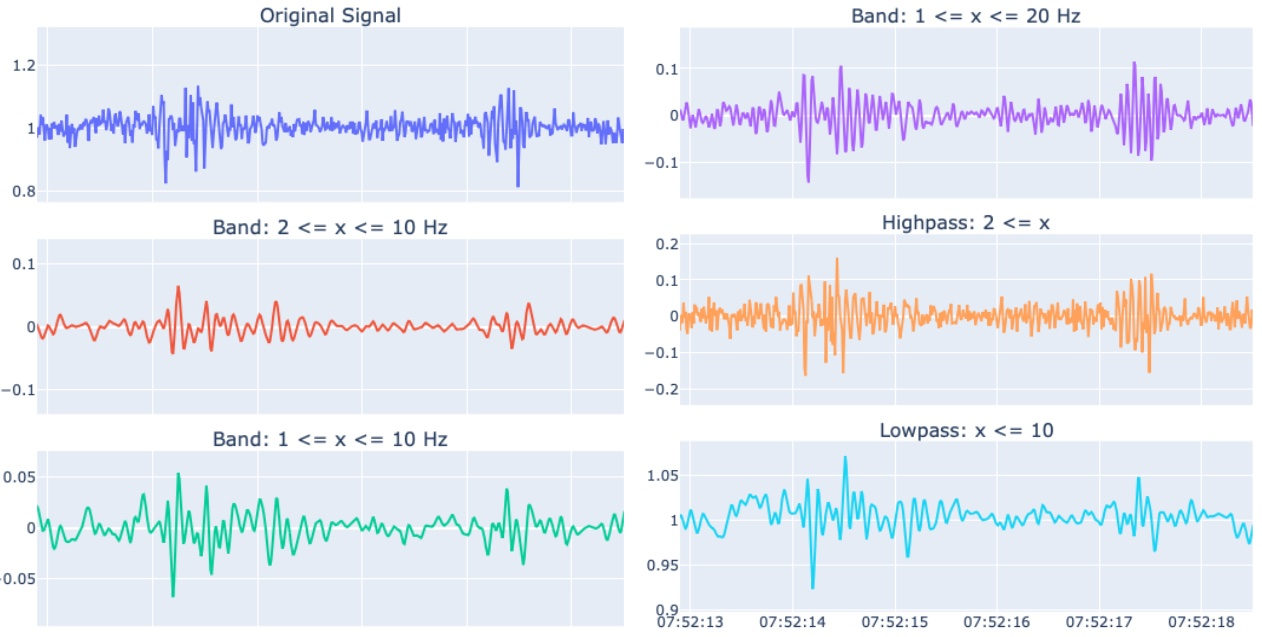
\includegraphics[width=0.95\textwidth,keepaspectratio]{images/4_data/filter-example.jpg}
\end{center}
\captionsetup{width=.90\textwidth}
\caption{Figure displaying various graphs after applying a 5th-order Butterworth filter to the accelerometer signal on the vertical Z-axis. The event shown here is when the vehicle drives over a manhole.}
\label{fig:filter}
\end{figure}




\subsection{Visual Data}
\label{sec:visual-data}

The road surface is recorded with an Apple iPhone 12 Mini. The data is recorded at resolution of 1280 x 720 at 30 frames per second (FPS). The phone is located in a generic  phone holder attached to the windshield. As can be seen in figure \ref{fig:smartphone-collector}, the camera records the road from front faced perspective. The camera collects also other data than the road e.g., other vehicles, the sky, and other surroundings. Below we describe the processing steps for the visual data. We anonymize such information before uploading it to the data platform. To this aim, these processing steps are ran on a local machine, as opposed to previous steps.

\begin{figure}[H]
\begin{center}

\includegraphics[width=0.95\textwidth,keepaspectratio]{images/4_data/visual-processing-steps.png}
\end{center}
\captionsetup{width=.90\textwidth}
\caption{Figure displaying all processing operations for visual data.}
\label{fig:processing-overview}
\end{figure}


\subsubsection{Video to Frames}
All visual data processing operations operate on single frames instead of video files. Therefore, the first step is to extract the distinctive frames from the video. We use the open-source FFmpeg \cite{ffmpeg} to convert a video into frames. Due the front faced perspective, the visual data contains a wide view of area. For instance, the horizon and the sky are also visible in the frame. Objects in the distance are smaller and more blurry making them harder to detect.

Therefore, we crop the exported frames to a smaller region where 1) there is less noise due surroundings, and 2) objects are more distinctive. Additionally, due the smaller image size, further computations are more efficient. The cropped area is selected as: the bottom half of the image, with an margin of 100 pixels from the bottom. With this margin we skip largely the area of the hood. Cropping of the frames is also implemented with the FFmpeg tool. An example is shown in figure \ref{fig:cropped-frame}, the red rectangle designates the cropped area. 

\begin{figure}[ht]
\centering
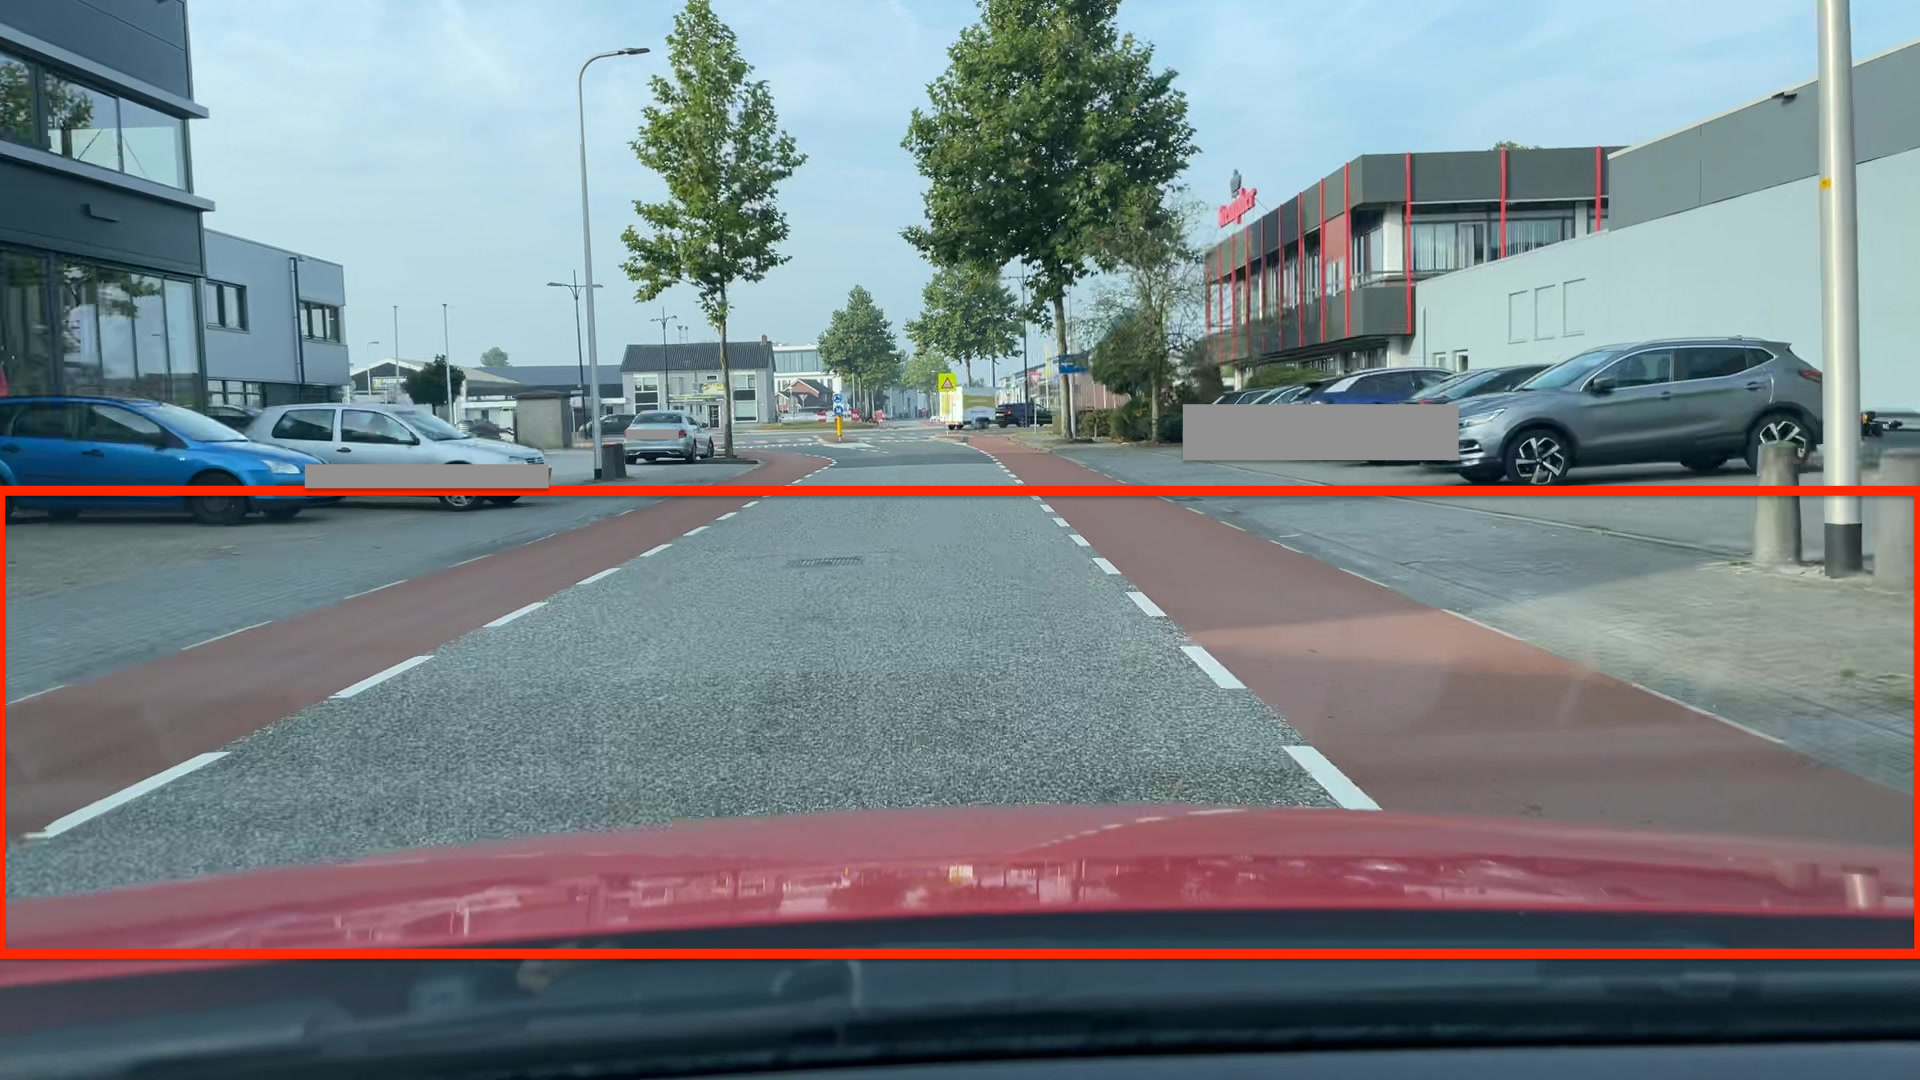
\includegraphics[width=0.85\textwidth,keepaspectratio]{images/4_data/crop-screenshot.png}
\captionsetup{width=.90\textwidth}
\caption{Figure showing one of the collected frames. The red rectangle designates the cropped area.}
\label{fig:cropped-frame}
\end{figure}



\subsubsection{Anonymization}
Although not intentional, the camera may record other cars, persons, and other PII data. To safeguard any privacy concerns, the data is anonymized by blurring PII data from the individual frames. Detection of PII data happens with pre-trained object detector YOLOv5 model \cite{Jocher2021}. This model is trained on the COCO dataset \cite{COCO}, and is capable of detecting various classes. The following classes are blurred: person, bicycle, car, motorcycle, bus, train, and truck. After the frames are anonymized, the frames are uploaded to the data platform.


% \subsubsection{Optical Flow}
% Visual and accelerometer data can be synchronized to distinguish events using both data. Dense optical flow estimates the acceleration between two frames and allows aligning visual and accelerometer data. See section \ref{sec:cross-correlation} for a detailed explanation. 

% For each of the extracted frames, we compute the optical flow by using the Farneback algorithm \cite{Farnebäck2003}. In this thesis we use the function \code{calcOpticalFlowFarneback} from the open-source image processing library OpenCV \cite{opencv}. For each frame, we compute the average of all flow pixels, which results in a 2D vector field, describing the motion of the frame in horizontal X- and vertical Y-axis. An pseudo implementation can be found in listing \ref{list:calculate_optical_flow}.

% Figure \label{fig:optical-flow} shows an example. At the top, the input frame is shown in the left, the right image is the output after calculating the optical flow. The bottom graphs compares the full vertical optical flow with that of measured accelerometer data. Although it is not visible in on this graph, there exists a small delay between the modalities due time synchronization. Referred to as $\tau_{capture}$. Synchronization of these modalities is tackled in section \ref{sec:capture-time-synchronization}.

% \begin{figure}[H]
% \centering
% \subfloat{{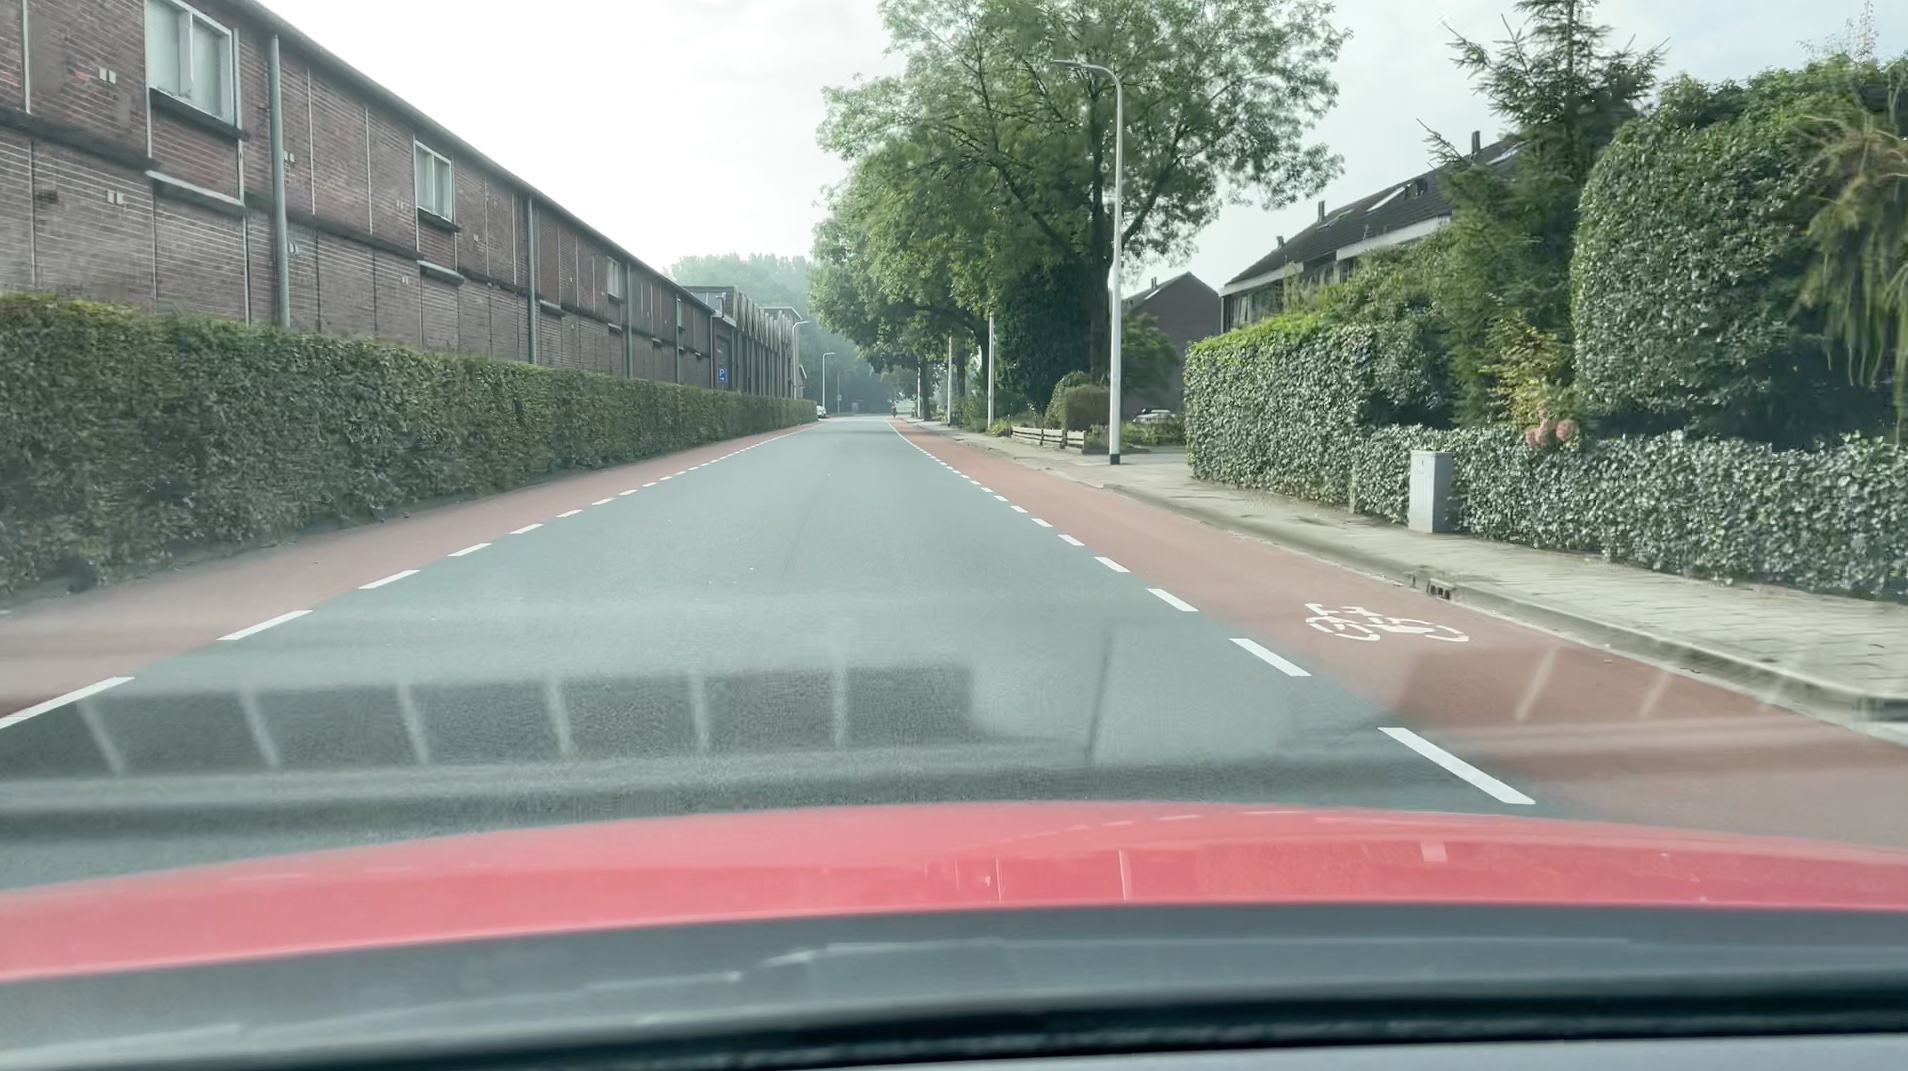
\includegraphics[width=0.45\textwidth,keepaspectratio]{images/4_data/original.jpg} }}%
% \quad
% \subfloat{{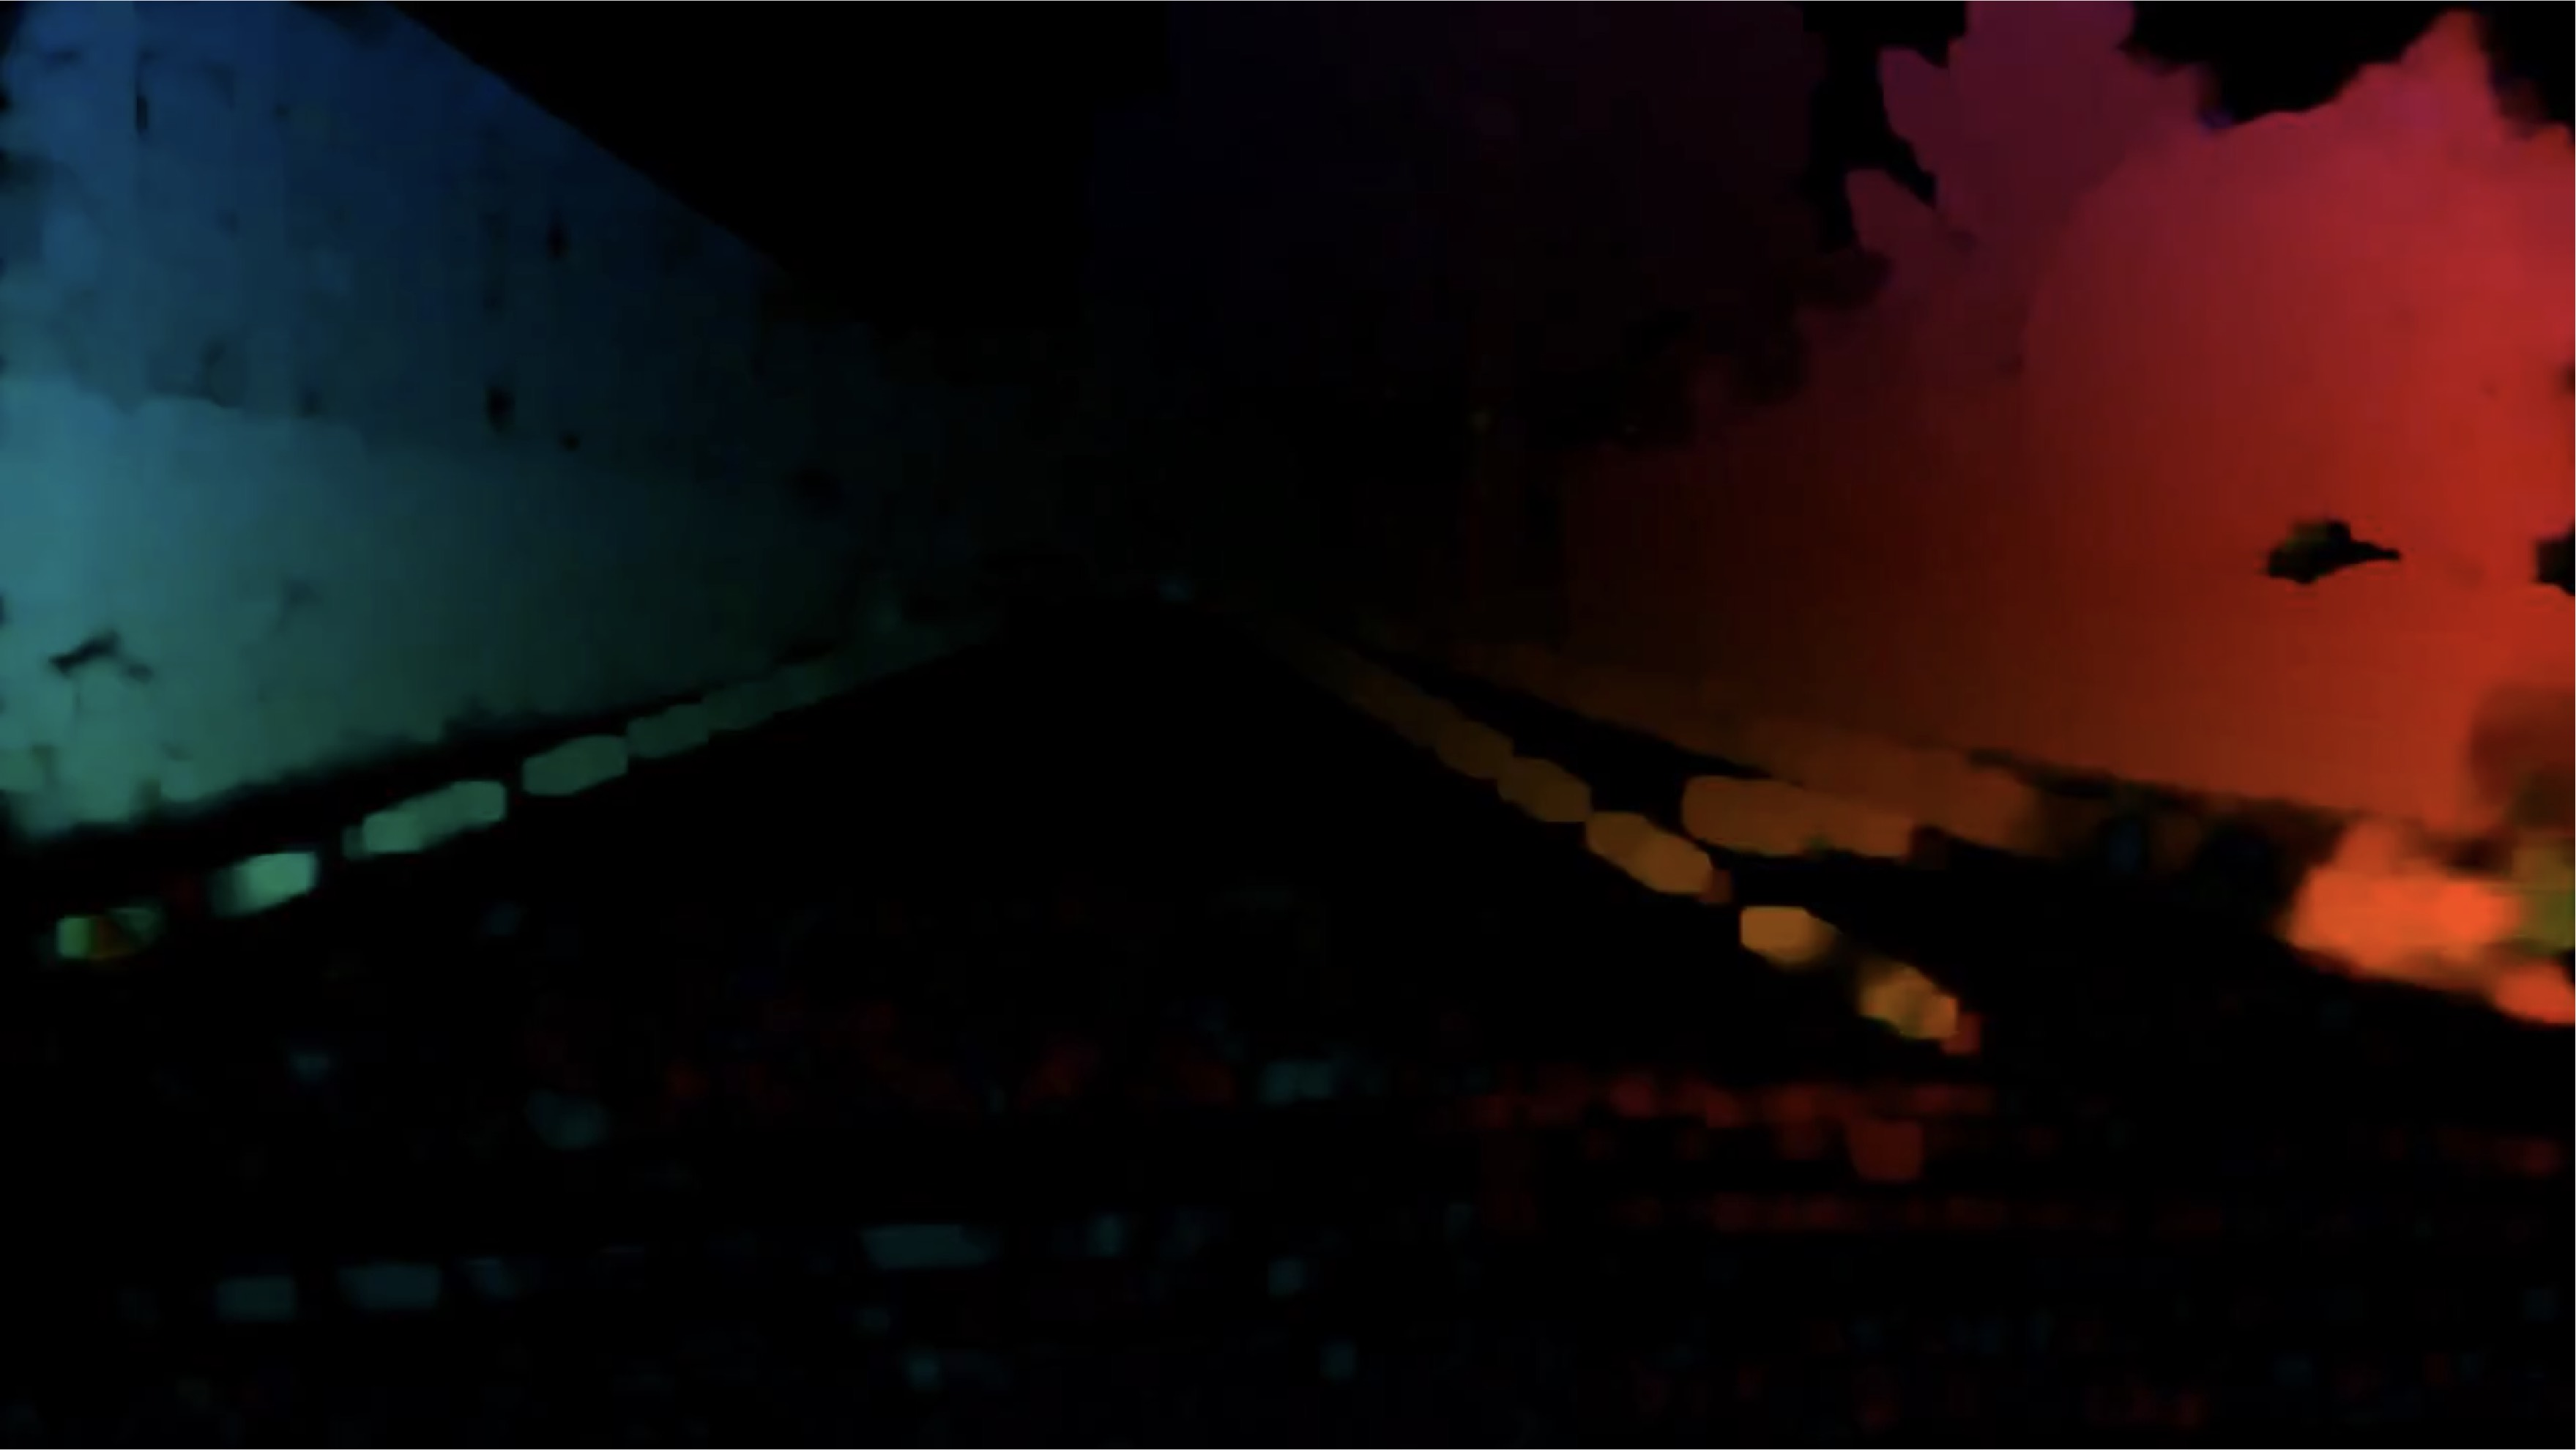
\includegraphics[width=0.45\textwidth,keepaspectratio]{images/4_data/optical-flow.jpg} }}%

% 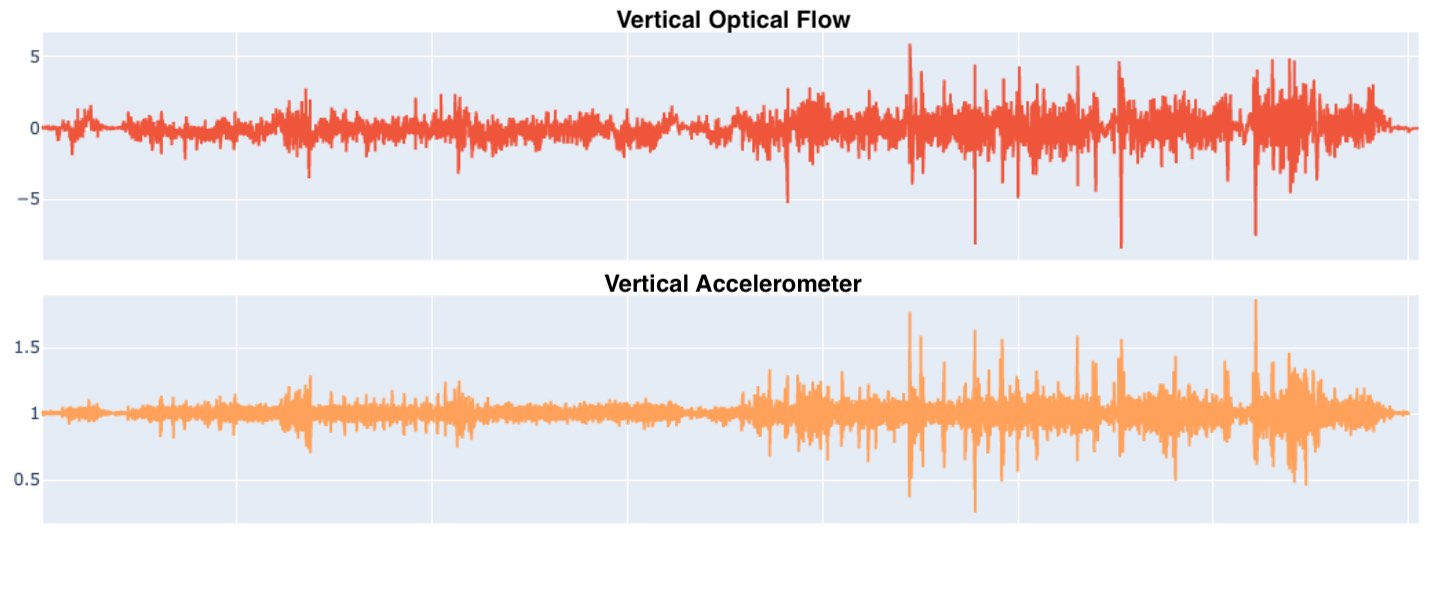
\includegraphics[width=0.95\textwidth,keepaspectratio]{images/4_data/optical-flow-graph.jpg}

% \captionsetup{width=.90\textwidth}
% \caption{At the top, the input frame is shown in the left, the right image is the output after calculating the optical flow. The bottom graphs compares the full vertical optical flow with that of measured accelerometer data.}
% \label{fig:optical-flow}
% \end{figure}


% \begin{minipage}{.95\textwidth}
% \begin{lstlisting}[language=Python, caption={Pseudo implementation of calculating optical flow from video.}, label={list:calculate_optical_flow}]
% def calculate_optical_flow(frames):
%     flow = []
    
%     previous = frames[0]
%     for frame in frames:
%         # Calculate flow for all pixels between two frames using
%         # farneback algorithm `\cite{opencv}`
%         flow_pixels = farneback(previous, current)
        
%         # Calculate average flow to describe motion in 2 axes
%         flow_x = mean(flow_pixels[..., 0])
%         flow_y = mean(flow_pixels[..., 1])
%         flow.append(flow_x, flow_y)
        
%         previous = frame
    
%     return flow
% \end{lstlisting}
% \end{minipage}



\subsubsection{Labelling}
\label{sec:visual-labelling}

As described earlier visual data is recorded with a smartphone at 30 frames per second. The visual data is manually annotated with open-source Computer Vision Annotation Tool (CVAT) \cite{cvat}.  Labelling of a frame is done by selecting all areas where a damage is present. See figure \ref{fig:cvat} for an example. Subsequently, the annotated data is exported and stored in the Data Platform. Note, annotating all frames is tedious as the change between between frames is minimal at 30 fps. Instead we downsampled the annotation to every tenth frame (i.e., 3 fps).


\begin{figure}[ht]
\centering
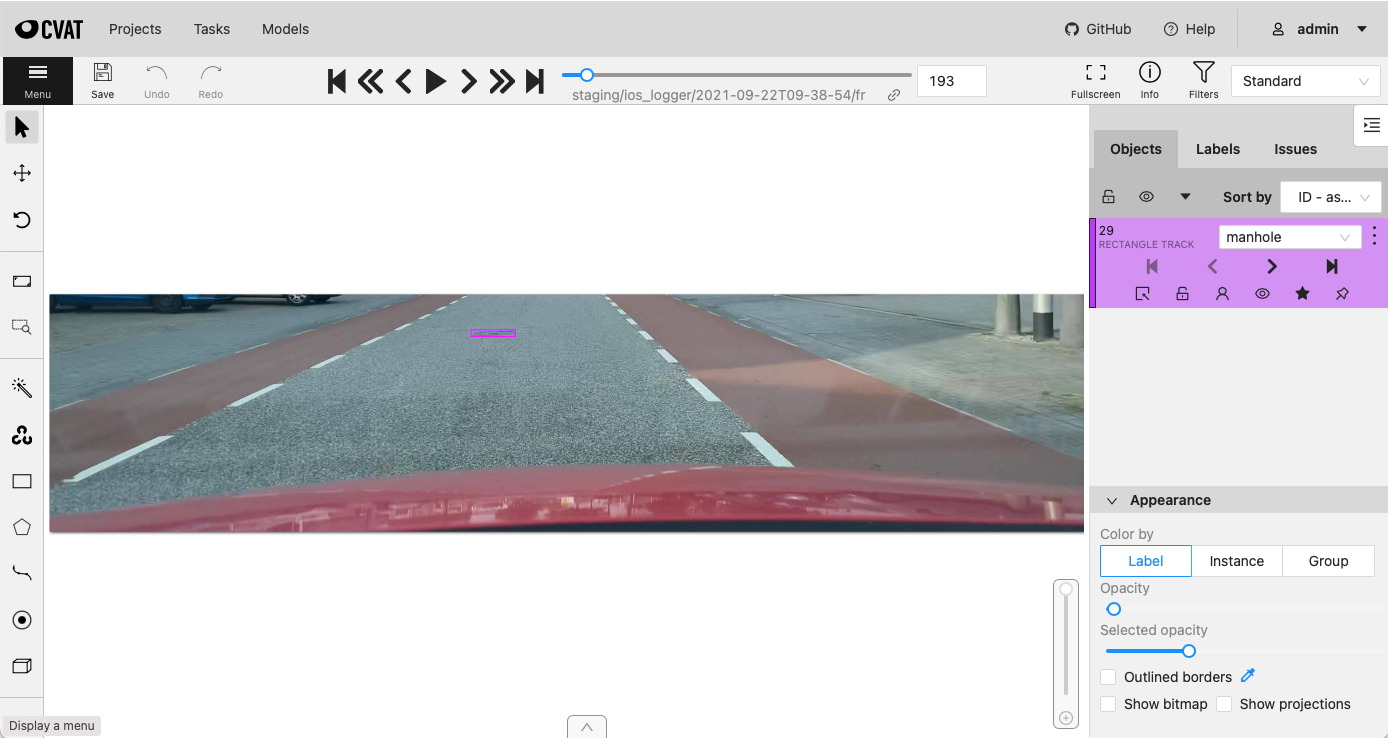
\includegraphics[width=0.95\textwidth,keepaspectratio]{images/4_data/cvat-screenshot.png}
\captionsetup{width=.90\textwidth}
\caption{Screenshot of the annotation tool CVAT \cite{cvat}.}
\label{fig:cvat}
\end{figure}


\subsection{Exploratory Data Analysis}

After applying the processing steps, we obtained a final dataset. The dataset consists of 17 trips, a total distance travelled over 246 km in 4 hours (average speed 62 km/h). The data is recorded over 10 different days. All data is collected in the Netherlands. A map of the travelled roads can be seen in figure \ref{fig:gps-trips}. Note, this includes only data collected with the smartphone approach. Data from the AutoPi is ignored as the accelerometer data is deemed unreliable.

\begin{figure}[ht]
\centering
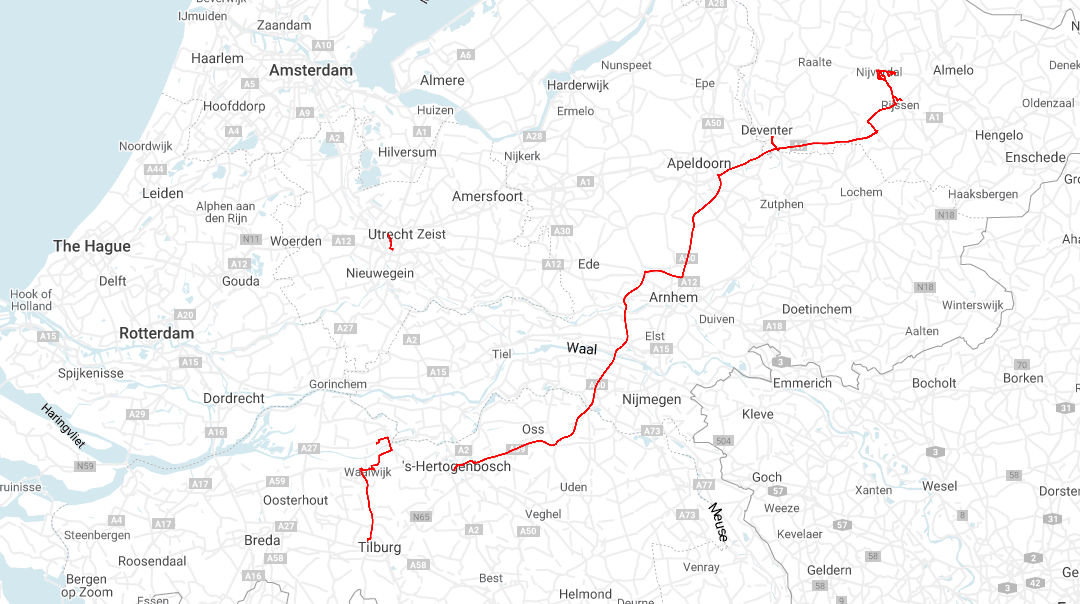
\includegraphics[width=0.8\textwidth,keepaspectratio]{images/4_data/gps-trips.png}
\captionsetup{width=.90\textwidth}
\caption{Map where the data is collected. The red lines indicates the coordinates travelled while collecting data.}
\label{fig:gps-trips}
\end{figure}

\subsubsection{Road Types}

To scope our research we only focus on detecting damages on asphalt roads. These types of roads cause less amount of vibrations than other types as roads (e.g., brick paved). These additional vibrations introduce additional noise for the accelerometer. When there is too much vibration, it is unlikely that the accelerometer is able to distinguish damages.

Additionally, brick paved roads are typically only used within urban areas. The majority of the roads (in Netherlands) are made from asphalt. Most types of damages are actually only present on asphalt roads. The proportion of road types per trip is shown in figure \ref{fig:proportion-road-types}. The type of road is determined by the BGT \cite{BGT}. 

\begin{figure}[ht]
\centering
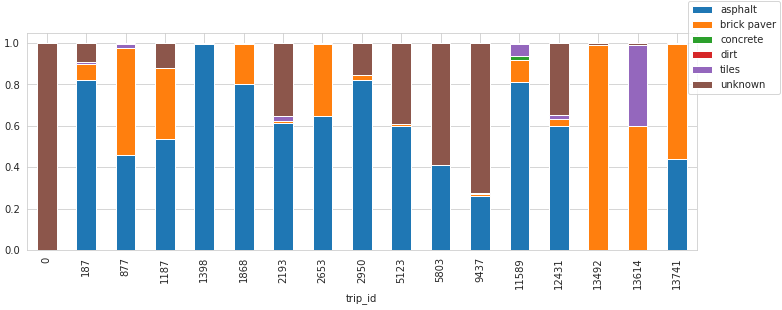
\includegraphics[width=0.8\textwidth,keepaspectratio]{images/4_data/proportion-road-types.png}
\captionsetup{width=.90\textwidth}
\caption{Proportion of the different road types per trip.}
\label{fig:proportion-road-types}
\end{figure}


\subsubsection{Labels}

As described, the visual data is manually annotated. We use these labels as ground truth when making predictions. In figure \ref{fig:distribution-labels} is shown the amount of labels per class. This illustrates a problem for our research. From the figure we observe that we have collected very few damages. Note, this figure includes the labelled data that was collected in combination with the AutoPi, i.e., data points where the accelerometer is unreliable. If we omit these labels, there are fewer damages.

To train a machine learning model we need many instances. However, with this few instances of damages it is impossible to train a model to detect road surface damages. The most prominent damage ``Road mark'' are faded road markings. This type of damage unlikely to be observed with the accelerometer, as the vehicle doesn't drive over road markings often. During the research period, efforts were made to discover more damages throughout the country. However, we argue that the current state of the Dutch infrastructure is in such decent condition it is infeasible to collect enough data in the limited time period of this study.

However, the developed methodology using multimodal machine learning can still be applied in this context. Instead of detecting road surface damages we apply the method to detect manholes. In Netherlands manholes are present everywhere on local roads. Additionally, they are often located at a place where the wheel path travels over. This makes manholes a suitable target for our method. In figure \ref{fig:distribution-labels}, the orange bar represent the amount of manholes annotated.

\begin{figure}[ht]
\centering
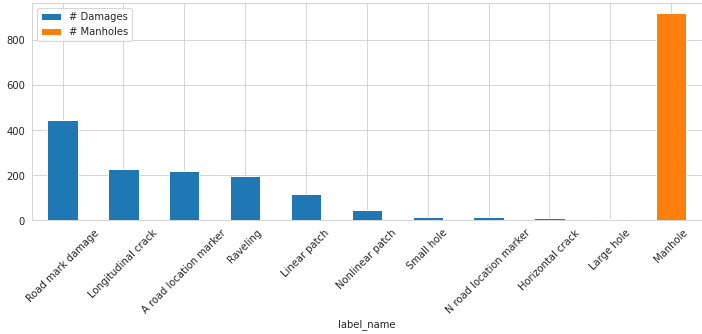
\includegraphics[width=0.8\textwidth,keepaspectratio]{images/4_data/label-counts.png}
\captionsetup{width=.90\textwidth}
\caption{Figure displaying the distribution of labels. Blue bars denote the amount of damages. Orange bar denote the amount of manholes.}
\label{fig:distribution-labels}
\end{figure}

